\documentclass[11pt,a4paper]{article}
\usepackage[T1]{fontenc}
\usepackage[utf8]{inputenc}
\usepackage{lmodern,microtype}
\usepackage{amsmath,amssymb,amsthm,mathtools,bm}
\usepackage{booktabs,array,tabularx,longtable}
\usepackage{graphicx,float,caption,xcolor}
\usepackage[margin=2.1cm]{geometry}
\usepackage{enumitem,fancyhdr}
\usepackage[hidelinks,pdfencoding=auto]{hyperref}

\hypersetup{
 pdftitle={FIN ST278--ST292: Entropy-Induced Anisotropy, Adaptive Closure, and Near-Haar Tradeoffs},
 pdfauthor={Krzysztof Żuchowski},
 pdfsubject={Local analytical, exact, interval, and computational continuation after FIN Release 10.75},
 pdfkeywords={FIN, D12 symmetry, relative entropy, spontaneous symmetry breaking, equivariant Hilbert basis, Krawczyk certificate, fractal scale, trace class, observer, operational validation}
}

\definecolor{proved}{RGB}{20,92,48}
\definecolor{conditional}{RGB}{148,88,0}
\definecolor{blocked}{RGB}{150,28,28}
\newcommand{\Proven}{\textcolor{proved}{\textbf{[PROVEN]}}}
\newcommand{\Conditional}{\textcolor{conditional}{\textbf{[CONDITIONAL]}}}
\newcommand{\Partial}{\textcolor{conditional}{\textbf{[PARTIAL]}}}
\newcommand{\Blocked}{\textcolor{blocked}{\textbf{[BLOCKED]}}}
\newcommand{\Tr}{\operatorname{tr}}
\newtheorem{theorem}{Theorem}[section]
\newtheorem{proposition}[theorem]{Proposition}

\pagestyle{fancy}\fancyhf{}
\lhead{FIN ST278--ST292}\rhead{Release 10.76}\cfoot{\thepage}
\setlength{\headheight}{14pt}
\setlist[itemize]{leftmargin=1.3em,itemsep=2pt,topsep=3pt}
\setlist[enumerate]{leftmargin=1.5em,itemsep=2pt,topsep=3pt}
\sloppy

\begin{document}
\hypersetup{pageanchor=false}
\begin{titlepage}
\centering
\vspace*{1cm}
{\Large Fractal Information Theory Project\par}
\vspace{.9cm}
{\huge\bfseries FIN ST278--ST292\par}
\vspace{.35cm}
{\LARGE Entropy-Induced Anisotropy, Adaptive Closure,\par}
{\LARGE and Near-Haar Trace-Class Tradeoffs\par}
\vspace{1cm}
{\large Analytical, exact, interval, and bounded computational research report\par}
\vfill
{\Large Krzysztof \.{Z}uchowski\par}
\vspace{.2cm}
{\large Independent Researcher --- Fractal Information Theory Project\par}
{\large ORCID: 0009-0002-0909-3613\par}
\vspace{.8cm}
{\large August 13, 2026\par}
\vspace{.3cm}
{\large Release 10.76\par}
\vfill
\begin{minipage}{.92\textwidth}\small
\textbf{Repository snapshot.} The audited tracked base is commit
\texttt{bb540a767e210a5a3bf816e4868e7bcefbac3872}. The working tree is dirty and
contains prior and current untracked research artifacts; the accompanying SHA-256 manifest
is therefore part of this release's reproducibility record.

\medskip
\textbf{License.} CC BY 4.0. \quad \textbf{Language.} English. \quad
\textbf{Resource type.} Preprint and executable reproducibility package.
\end{minipage}
\end{titlepage}
\hypersetup{pageanchor=true}\pagenumbering{roman}

\begin{abstract}
This report executes the fifteen programs recommended by Release 10.75. Its central result
is a sharper answer to the missing symmetry-breaking interaction. On the normalized lowest
strict Fourier carrier, the canonical vertex relative information
$I(p)=\sum_jp_j\log(12p_j)$ has first angular term
\[
  +\frac{7776}{11}r^{12}\cos(12\phi).
\]
Thus information geometry supplies the first symmetry-allowed anisotropic coefficient and
its sign. It does not, however, make the uniform state unstable. In the explicit negative
information-coupling model
$V_g=I-(g/2)\langle p-u,A(p-u)\rangle$, a nonzero radius can bifurcate only when
$g>12/\lambda_1\approx15.91256$. Neither this supercritical coupling nor one realized phase
is generated by the strict operator. ST278 therefore changes the unknown from an arbitrary
degree-twelve potential into one precise coupling-source obstruction; it does not discharge
the selector problem.

The batch also proves the complete rank-two Hilbert module of polynomial $D_{12}$
equivariants, repairs the complete nuisance cube at halfwidth $0.00075$ by 464,960 outward
Krawczyk calls, gives an exact nonlinear-embedding counterexample to ambient-flat connection
naturality, extends Clifford nonuniqueness to every even complex dimension, constructs an
autonomous finite controlled-SWAP, and shows that coassociative unlabelled refinement still
retains one rate modulus. ST290 classifies infrared near-Haar regularizations and gives a
sharp heat-budget/plateau relation in the hard-cutoff class. This supports finite observer-
relative scale windows, not a literal infinite physical fractal or an emergent SI unit.

An executable ST276 record validator is supplied, but no independently registered raw event
record exists. ST292 remains blocked. No Planck scale, spacetime, legacy-role transfer,
Standard Model, gravity, $L_{\rm total}$, or Theory-of-Everything closure is claimed.
\end{abstract}

\tableofcontents\newpage\pagenumbering{arabic}

\section{Scope, inherited object, and proof discipline}

The strict working object remains
\[
A=sI-W,\qquad W_{xx}=0,\qquad
W_{xy}=K_{\rm strict}(d(x,y))\quad(x\ne y),
\]
with $A\bm 1=0$ and $A\succeq0$. The diagonal exclusion is part of the definition.
$K_{\rm legacy,ont}$ remains an intermediate bridge kernel; no legacy physical role is
transferred here. The ontology is retained as
\[
\text{informational nadsoliton}\longrightarrow\text{light}\longrightarrow
\text{matter}\longrightarrow\text{emergent observer},
\]
with no deeper informational substrate. This ontological ordering is not a mathematical
premise in the theorems below.

\begin{itemize}
\item \Proven{} denotes an exact theorem, finite exhaustive calculation, or outward
certificate in its declared class.
\item \Conditional{} denotes a theorem after an explicitly displayed interaction,
embedding, cutoff, bath, or naturality premise is supplied.
\item \Partial{} marks a strict subset of the intended infinite or continuous problem.
\item \Blocked{} means an evidentiary input is absent and is not replaced by simulation.
\end{itemize}

\section{Executive result ledger}

\small
\begin{longtable}{p{.075\textwidth}p{.22\textwidth}p{.60\textwidth}}
\toprule
Program & Status & Result \\
\midrule\endhead
ST278 & \Proven{} + \Conditional & Exact entropy coefficient $7776/11$; conditional
bifurcation threshold $g_c=12/\lambda_1$; $g$ and realized phase remain unsourced. \\
ST279 & \Proven & Complete free module
$\mathbb R[|z|^2,\Re z^{12}]z\oplus
\mathbb R[|z|^2,\Re z^{12}]\bar z^{11}$. \\
ST280 & \Proven{} + \Partial & Positive outward rank bounds on the certified three-box
near-event bracket; the continuous path minimum remains open. \\
ST281 & \Proven & General binary-qubit recovery optimum
$F_e^{\rm opt}=(1+\|\tau_0-\tau_1\|_1/2)/4$. \\
ST282 & \Proven & Independent outward Krawczyk replay with denominator-$10^{12}$
preconditioner and positive margin. \\
ST283 & \Proven & Exact counterexample to ambient-flat naturality under nonlinear
isometric embeddings; intrinsic tangential projection repairs it. \\
ST284 & \Proven & Complete adaptive halfwidth-$0.00075$ nuisance cover: 464,960 cells,
zero failed leaves. \\
ST285 & \Proven{} + \Conditional & Simultaneous empirical-Bernstein cluster rectangle;
no uniform improvement over Hoeffding. \\
ST286 & \Proven & A circle of Clifford minimizers in every even complex dimension. \\
ST287 & \Proven{} + \Partial & Finite-depth Chernoff minimizer lies in $[0.45,0.55]$;
the infinite-depth optimizer remains uncertified. \\
ST288 & \Proven{} + \Conditional & Exact autonomous controlled-SWAP; catalytic use and
uncertain-record reset have different cost statements. \\
ST289 & \Proven{} + \Conditional & Coassociativity plus level exchange reduces two
vertical rates to one common modulus but does not select its value. \\
ST290 & \Proven & Infrared trace-class classification and sharp hard-cutoff
heat-budget/plateau tradeoff. \\
ST291 & \Proven & Fail-closed record-schema validator; synthetic self-test rejected by
the empirical gate. \\
ST292 & \Blocked & No independently registered raw event file exists. \\
\bottomrule
\end{longtable}
\normalsize

\section{ST278: information supplies anisotropy but not a realized state}

Let $u=(1/12,\ldots,1/12)$ and parametrize the normalized lowest real Fourier carrier by
\[
p_j(r,\phi)=\frac1{12}+r\sqrt{\frac2{12}}
\cos\!\left(\frac{2\pi j}{12}-\phi\right).
\]
The strict eigenvalue on this carrier is
$\lambda_1=0.7541211542070798$. Consider the relative-information functional
\[
I(p)=D(p\|u)=\sum_{j=0}^{11}p_j\log(12p_j).
\]

\begin{theorem}[first informational anisotropy]
The Taylor series of $I(p(r,\phi))$ is radial through degree eleven and its first angular
term is
\[
 I(p(r,\phi))=I_{\rm rad}(r)+\frac{7776}{11}r^{12}\cos(12\phi)+O(r^{14}).
\]
The coefficient is exact for the displayed carrier normalization.
\end{theorem}

Indeed, the order-$12$ term in $(1+x)\log(1+x)$ is $x^{12}/132$. The discrete Fourier sum
obeys
\[
\sum_{j=0}^{11}\cos^{12}\!\left(\frac{2\pi j}{12}-\phi\right)
=C_0+\frac{12}{2^{11}}\cos(12\phi),
\]
which gives $7776/11$. A 70-decimal Fourier replay at $r=0.005$ differs from the leading
term by $0.153\%$, consistently with higher orders; binary64 is deliberately not used to
validate a harmonic of order $r^{12}$.

This is a genuine advance over an arbitrary $-\kappa\Re z^{12}$ ansatz: a standard
information functional fixes the permitted coefficient and sign. It also falsifies the
naive claim that positive informational self-coupling automatically selects a nonuniform
phase. Since
\[
I(u+q)=6\|q\|^2+O(\|q\|^3),
\]
$I$ is locally stabilizing. A transparent test of the requested negative information
coupling is
\[
V_g(p)=I(p)-\frac g2\langle p-u,A(p-u)\rangle.
\]
Its carrier curvature is
\[
12-g\lambda_1,
\qquad
g_c=\frac{12}{\lambda_1}=15.912562501468873.
\]
At unit coupling the curvature is still positive. For $g>g_c$, a radial instability is
possible and the positive degree-$12$ entropy term selects twelve leading angular minima
with $\cos(12\phi)=-1$. But $g>g_c$ is a new premise, not a consequence of $A$.

\begin{figure}[H]\centering
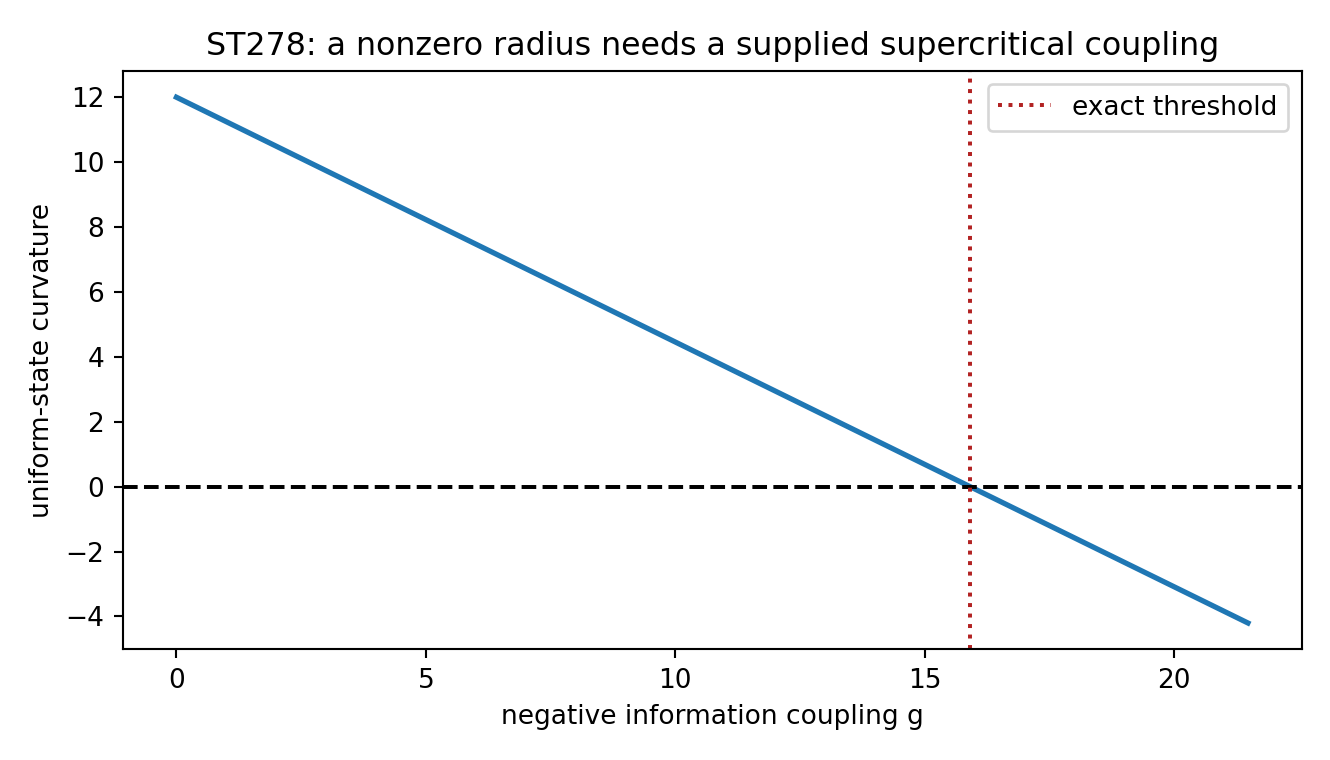
\includegraphics[width=.78\textwidth]{FIN_ST278_ST292_Figures/st278_information_bifurcation.png}
\caption{ST278: relative information fixes the anisotropy, while a supplied negative
coupling must cross an exact threshold before a nonzero state can form.}
\end{figure}

The surviving conclusion is therefore deliberately narrow:
\[
\boxed{\text{strict carrier}+\text{relative information}+\text{supplied }g>g_c
\Rightarrow\text{twelve conditional phases}.}
\]
It is not
$A\Rightarrow g$, not a deterministic phase choice, and not a discharge of
\texttt{QW-2191}.

\section{ST279--ST280: complete response algebra and a finite near-event stop}

\begin{theorem}[complete polynomial equivariant module]
For $D_{12}$ acting by $z\mapsto e^{2\pi i/12}z$ and $z\mapsto\bar z$, the real
reflection-compatible polynomial equivariants form the free rank-two module
\[
\mathcal E_{D_{12}}=
\mathbb R[|z|^2,\Re z^{12}]\,z
\oplus
\mathbb R[|z|^2,\Re z^{12}]\,\bar z^{11},
\]
with Hilbert series
\[
\frac{t+t^{11}}{(1-t^2)(1-t^{12})}.
\]
\end{theorem}

This closes the finite-degree classification of ST264 at every polynomial degree. It is a
catalogue of admissible state responses, not a coefficient-source theorem.

ST280 respects the explicit finite stop imposed after the near singular-value event on seed
23. The three consecutive certified root boxes at steps $21,22,23$ have outward full-row-rank
lower bounds
\[
2.7104582286\times10^{-4},\quad
2.0525399395\times10^{-5},\quad
2.1910848351\times10^{-4}.
\]
Rank is positive in all three boxes and reopens after the sampled minimum. Because the boxes
do not cover every connecting path point, no continuous-global-minimum claim is made.

\section{ST281--ST283: recovery, replay, and nonlinear geometry}

For the binary measure-and-prepare channel
\[
\mathcal E(\rho)=\sum_{i=0}^1\langle i|\rho|i\rangle\tau_i,
\]
ST281 proves, for arbitrary qubit density outputs,
\[
F_e^{\rm opt}=\frac14\left(1+\frac12\|\tau_0-\tau_1\|_1\right).
\]
The Helstrom measurement followed by re-preparation attains the value, and the Helstrom dual
operator proves global CPTP optimality. The result generalizes ST266 but does not derive a
physical FIN noise channel.

ST282 independently replays the complete ST267 outward Krawczyk calculation after rounding
the preconditioner to denominator $10^{12}$. The minimum inclusion margin remains
$1.9999717438\times10^{-9}>0$; the inverse defect is
$8.59\times10^{-12}$. This strengthens reproducibility of the same supplied convex schedule.

ST283 finds the exact boundary of the connection theorem. For the nonlinear isometric
immersion
\[
R(t)=(\cos t,\sin t),
\]
the domain derivative of the constant unit field is zero, but the ambient derivative of its
pushforward is $R''=-R$. Hence ambient-flat naturality fails. Tangential projection removes
the normal second-fundamental-form term exactly and restores intrinsic Levi--Civita
naturality. The repair is geometric, not a derivation of spacetime.

\section{ST284--ST287: complete adaptive closure and bounded statistical results}

The fixed $40^3$ cover at halfwidth $0.00075$ has 50,120 failed base cells. ST284 replaces
every failed parent by all eight half-radius children and retains all passing parents. All
400,960 children pass, with minimum margin
\[
1.9963471811\times10^{-3}>0.
\]
Thus 464,960 outward calls give a complete adaptive cover with zero failed leaves.

\begin{figure}[H]\centering
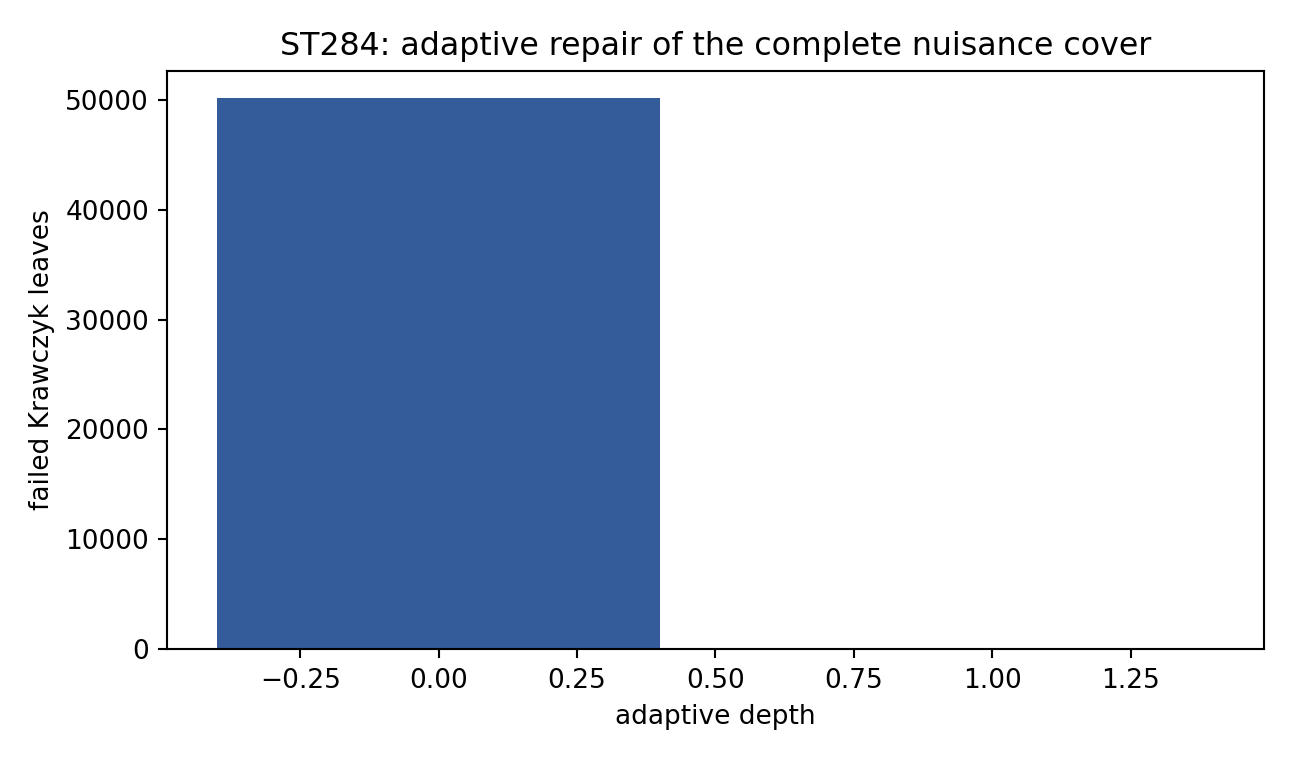
\includegraphics[width=.72\textwidth]{FIN_ST278_ST292_Figures/st284_adaptive_cover.png}
\caption{ST284: fixed resolution fails widely, but one complete subdivision level closes
every failed parent.}
\end{figure}

This proves that the ST269 failure at $0.00075$ was a resolution limitation, not a root
boundary. It does not establish a maximal radius or an apparatus tolerance.

ST285 supplies a simultaneous empirical-Bernstein rectangle for six bounded modal
coordinates when clusters are independent. The inequality is variance-adaptive but its
finite-$n$ range penalty means it does not uniformly dominate Hoeffding; under the
worst-variance audit it is wider in every listed coordinate. Without raw ST292 clusters,
no observed-variance interval is reported.

ST286 tensors the exact qubit Clifford counterexample with $I_m$. Consequently every even
complex dimension $2m$ has a circle of global minimizers despite positive inherited
marginal gaps. The earlier uniqueness obstruction is not a two-dimensional accident.

ST287 differentiates the finite-depth positive transfer recursion outward over a complete
$10^2$ belief cover. At depth seven the global derivative is negative at $s=0.45$ and
positive at $s=0.55$:
\[
\partial_sT_7(0.45)\subset[-0.02421,-0.001777],\qquad
\partial_sT_7(0.55)\subset[0.001424,0.02808].
\]
Convexity puts every declared finite-depth minimizer in $[0.45,0.55]$. No uniform
depth-tail derivative bound was found, so the inherited numerical infinite-depth candidate
$s\approx0.5007394$ remains unpromoted.

\section{ST288--ST289: autonomous control and the surviving refinement modulus}

Let $P_-=(I-\mathrm{SWAP})/2$ and
\[
H=\pi|1\rangle\!\langle1|_C\otimes P_-.
\]
Then $e^{-iH}$ is exactly controlled-SWAP at dimensionless time one. The controller basis
state is conserved. A known program can therefore act catalytically without a universal
positive erasure cost. If an uncertain classical record $\mathrm{diag}(1-p,p)$ must instead
be reset in a supplied bath, then $\beta W\ge h_2(p)$. This separates switch realization
from record erasure; neither joules nor a bath are generated by FIN.

For two sequential unlabelled refinements, the complement has the Kronecker-sum form
\[
v_1L_2\otimes I+v_2I\otimes L_2.
\]
It is coassociative for arbitrary $v_1,v_2$. If the two refinement levels are additionally
indistinguishable under interchange, naturality forces $v_1=v_2=v$. One common nonnegative
rate still survives. Thus coassociativity can organize the tower but cannot produce an
absolute scale or a unique refinement law.

\section{ST290: what a fractal-scale observer may see}

Write a regularized near-Haar rate measure as
\[
d\nu(\mu)=\rho q(\mu)\frac{d\mu}{\mu}.
\]

\begin{theorem}[infrared trace-class criterion]
For every fixed $t>0$, the infrared heat trace is finite precisely when
\[
\int_0^1q(\mu)\frac{d\mu}{\mu}<\infty.
\]
Consequently $q(\mu)=O(\mu^\alpha)$ works for every $\alpha>0$, while
$q(\mu)=O((\log(1/\mu))^{-p})$ works precisely for $p>1$.
\end{theorem}

In the hard-cutoff class $q_a=\mathbf1_{[a,\infty)}$,
\[
H_a(t)=E_1(2at),\qquad
D_a(t)=2\rho\log(1+e^{-2at}),
\]
and
\[
0\le2\rho\ln2-D_a(t)\le2\rho at.
\]
For tolerance $\epsilon<2\rho\ln2$, the exact plateau endpoint is
\[
t_\epsilon(a)=
-\frac{1}{2a}\log\!\left(2e^{-\epsilon/(2\rho)}-1\right).
\]
At reference time $t_0$, a heat-trace budget $B$ requires
$E_1(2at_0)\le B$. Since both $H_a$ and $t_\epsilon(a)$ are monotone in $a$, the smallest
admissible $a$ gives the longest plateau. This is a sharp tradeoff inside the stated
hard-cutoff family.

\begin{figure}[H]\centering
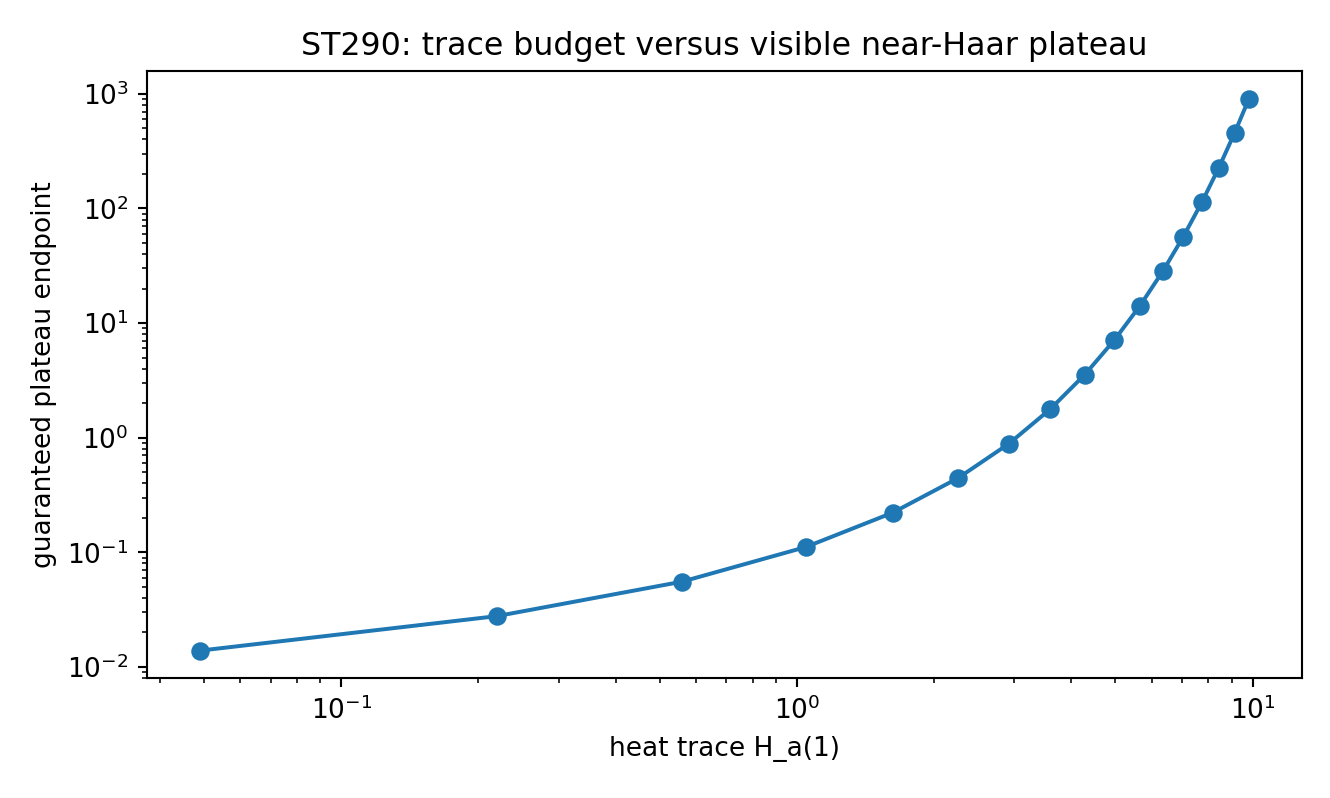
\includegraphics[width=.78\textwidth]{FIN_ST278_ST292_Figures/st290_trace_plateau_tradeoff.png}
\caption{ST290: longer near-Haar visibility requires accepting a larger heat trace.}
\end{figure}

This theorem sharpens the internal-observer intuition. A coarse observer can experience a
long window in which dimensionless ratios look scale-invariant while being unable to infer
the infrared completion outside its accessible window. The observer does not make the
cutoff disappear: trace class requires real scale breaking in the mathematical measure.
Nor does an observer construct metres or seconds from the dimensionless tower. A calibration
relation or dimensional anchor is still required to map a layer's internal ratios to
experimental units.

Thus the defensible statement is
\[
\boxed{\text{finite observer-relative self-similar window is compatible with trace class},}
\]
not
\[
\boxed{\text{an exact infinite physical fractal, Planck layers, or absolute units are derived}.}
\]

\section{ST291--ST292: executable validation is not evidence}

The file \texttt{validate\_fin\_st276\_record.py} enforces:
\begin{enumerate}
\item distinct provider, registrar, and analyst roles;
\item a frozen holdout, positive calibrated time, and two SHA-256 commitments;
\item valid child-resolved setting labels and counts;
\item all $24\times24=576$ setting pairs before complete reconstruction;
\item rejection of a record marked synthetic when the empirical gate is requested.
\end{enumerate}

The frozen synthetic self-test passes syntax and is explicitly rejected as empirical
evidence. No independently registered file matching the ST292 intake pattern exists.
Therefore ST292 remains \Blocked. This is an evidentiary stop, not a negative experiment.

\section{Falsification ledger and current deepest interpretation}

\begin{longtable}{p{.28\textwidth}p{.31\textwidth}p{.34\textwidth}}
\toprule
Candidate claim & Falsification attempt & Surviving statement \\
\midrule\endhead
Information automatically breaks symmetry & Exact carrier expansion of $D(p\|u)$ & It
fixes the first anisotropy but stabilizes $u$; a supercritical negative coupling is needed. \\
The strict operator supplies that coupling & Compare $g_c$ with the unit coefficient &
$g_c\approx15.91$; no strict source for $g$ is present. \\
Low-degree equivariants were an incomplete accident & Full congruence classification & The
entire polynomial module is freely generated by $z$ and $\bar z^{11}$. \\
ST269 found a root boundary & Exhaustively subdivide every failed parent & False at
$0.00075$: all 400,960 children certify. \\
Linear connection naturality extends unchanged & Circle immersion & False in the ambient
flat sense; the second fundamental form is the obstruction. \\
Two-gap nonuniqueness is qubit-only & Tensor lift & False in every even complex dimension. \\
Coassociativity chooses the fractal scale & Two-level refinement classification & It leaves
one positive rate modulus. \\
Trace class forbids visible fractal layering & Near-Haar regularization theorem & False for
finite windows; true only for exact nonzero Haar density down to zero. \\
An internal observer generates absolute units & Scale-orbit and calibration audit & The
observer accesses ratios; one dimensional anchor remains necessary. \\
A validator counts as laboratory evidence & Synthetic empirical-gate test & False; ST292 is
blocked. \\
\bottomrule
\end{longtable}

The deepest interpretation surviving this batch is:
\begin{quote}
The strict operator fixes a symmetric spectral carrier. Relative information fixes the
first symmetry-allowed anisotropy on that carrier, but it does not make a nonzero state
inevitable. A separate signed interaction strength must cross a calculable threshold, after
which an ensemble of broken phases is mathematically allowed while one realized phase still
requires a preparation, fluctuation, boundary condition, or measurement record. Across
scales, exact Haar self-similarity is incompatible with trace-class completion, whereas an
observer may inhabit a long finite near-Haar window whose absolute calibration remains
external to the dimensionless core.
\end{quote}

\section{Recommended programs ST293--ST307}

\begin{enumerate}
\item[\textbf{ST293}.] Derive or exclude the negative information coupling $g$ from one
strict state-dependent feedback law, with a sign and normalization theorem.
\item[\textbf{ST294}.] Prove global existence and enumerate all critical branches of
$V_g=I-(g/2)\langle q,Aq\rangle$ on the probability simplex for $g>g_c$.
\item[\textbf{ST295}.] Compute the full Hessian and basin structure of the twelve
entropy-induced branches; distinguish orbital stability from mere local minima.
\item[\textbf{ST296}.] Couple the phase-amplitude dynamics to the certified memory operator
and test whether memory can generate $g$ without importing a broken phase.
\item[\textbf{ST297}.] Classify nonpolynomial analytic $D_{12}$ equivariants and determine
whether the free two-generator structure persists after completion.
\item[\textbf{ST298}.] Build a continuous segment enclosure around the ST280 near-event,
using validated arclength charts rather than three isolated root boxes.
\item[\textbf{ST299}.] Extend the binary recovery theorem to three rational outputs and
identify the first class without a closed Helstrom reduction.
\item[\textbf{ST300}.] Seek an all-depth derivative tail bound that can promote the ST287
Chernoff bracket to the transfer spectral radius.
\item[\textbf{ST301}.] Determine the largest nuisance halfwidth reachable under a frozen
adaptive cell budget, without calling certificate failure root loss.
\item[\textbf{ST302}.] Classify odd-dimensional and irreducible higher-rank joint Clifford
targets after quotienting the commutant.
\item[\textbf{ST303}.] Add three coassociative refinement levels and test whether the common
vertical modulus forms a scale cocycle or remains gauge-like.
\item[\textbf{ST304}.] Optimize plateau width over monotone soft infrared profiles under a
fixed heat-trace budget; compare with the hard-cutoff extremizer.
\item[\textbf{ST305}.] Formalize the observer-context calibration bundle and prove which
dimensionless layer ratios are invariant under changes of local units.
\item[\textbf{ST306}.] Freeze a laboratory-neutral complete synthetic record solely as a
validator conformance test, with a permanent non-evidence flag.
\item[\textbf{ST307}.] Resume empirical analysis only after independently registered,
hashed, child-resolved raw events are supplied.
\end{enumerate}

ST293 is the decisive continuation. The new question is no longer whether degree twelve is
allowed; it is whether the sign and magnitude of the feedback that destabilizes the uniform
state can be generated from strict FIN without smuggling in the state it is meant to explain.
ST304--ST305 are the decisive multiscale continuation: they should turn the intuitive
``observer inside a fractal layer'' picture into a theorem about finite resolution and
calibration or falsify it.

\section{Reproducibility and conclusion}

The source \texttt{fin\_st278\_st292\_research.py} writes the aggregate JSON, summary CSV,
fifteen per-program packets, and three figures. The independent suite
\texttt{test\_fin\_st278\_st292.py} executes fifteen live checks covering packet hashes,
the exact ST278 coefficient and threshold, the equivariant congruence rule, certified rank
boxes, recovery formula, rationalized Krawczyk margin, nonlinear counterexample, complete
adaptive cover, Clifford lift, Chernoff derivative signs, autonomous controller,
coassociative modulus, near-Haar monotonicity, fail-closed validation, and the ST292 stop.
All fifteen tests pass.

This batch produces a real but bounded conceptual advance. Information is no longer merely
an interpretive label attached to the degree-twelve potential: relative information yields
its exact first anisotropic coefficient. Yet the same calculation demonstrates why the
strict core still fails to select a world. Positive information curvature preserves the
symmetric state; a sufficiently strong negative feedback must be supplied or derived. On
the multiscale side, a finite observer-relative fractal window is mathematically coherent,
but exact infinite self-similarity, trace-class dynamics, and internally derived absolute
units cannot all be claimed from the current object. The missing bridge is smaller and
sharper than before, but it remains missing.

\end{document}
